\subsection{Esercizio 7}
Le nuove funzioni utilizzate in  questo esercizio sono:
\begin{itemize}
    \item Metodo di Newton modificato
    \lstinputlisting[language=Matlab]{capitolo2/newtonmod.m}
    \item Metodo delle accelerazioni di Aitken
    \lstinputlisting[language=Matlab]{capitolo2/aitken.m}
\end{itemize}
La radice nulla della funzione $f(x)=x^2tan(x)$ ha molteplicità m = 3, in quanto $0$ annulla due volte il termine
$x^2$ e una volta il termine $tan(x)$. 


\begin{table}[h]
    \renewcommand\arraystretch{2}
    \begin{tabular}{|l l l l|}
            \hline
            Tolleranza &  Newton & Newton modificato & Aitken  \\
            \hline
            $10^{-3}$  &1.99400296195610$\cdot10^{-3}$ &1.32348898008484$\cdot10^{-23}$ & 3.72603946110722$\cdot10^{-24}$  \\
            $10^{-6}$  & 1.34922220938115$\cdot10^{-6}$ &1.32348898008484$\cdot10^{-23}$& 3.72603946110722$\cdot10^{-24}$ \\
            $10^{-9}$ &1.36940553054800$\cdot10^{-9}$&           0       & 2.93579661656743$\cdot10^{-39}$ \\
            $10^{-12}$ & 1.38989077859525$\cdot10^{-12}$ &       0             &2.93579661656743$\cdot10^{-39}$\\
            \hline
    \end{tabular}
    \caption{valori approssimati da newton, newton modificato e aitken(dati raccolti in \nameref{cod:7})}
    \label{tab::2}     
    \end{table}
\newpage    
\begin{figure}[h]
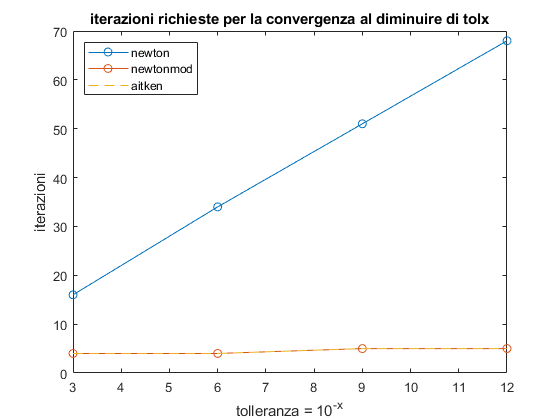
\includegraphics[scale=0.7]{capitolo2/iter2.png}
\caption{iterazioni richieste}
\label{fig::es6}
\end{figure}
Il metodo di newton classico perde la convergenza quadratica, essendo la radice cercata di molteplicità multipla. Il metodo di newton modificato e il metodo di aitken convergono
molto più rapidamente e newton modificato riesce anche a trovare la radice esatta.